% !TeX program = lualatex
% !TeX root = luaking.tex
% !TeX encoding = UTF-8
% !TeX spellcheck = cs_CZ
%---------------------------------------------------------------------------------------------------
% file fey1ch20.tex
%---------------------------------------------------------------------------------------------------
%=========================== Kapitola: Rotace v prostoru ===========================================
\setchaptertoc
\chapter{Rotace v prostoru}\label{fyz:IchapXX}
  \section{Momenty sil v prostoru}\label{fyz:IchapXXsecI}
    V této kapitole se budeme zabývat jedním z nejpozoruhodnějších a nejzábavnějších důsledků
    mechaniky - chováním rotujícího tělesa. Za tím účelem musíme nejdříve rozšířit matematickou
    formulaci rotačního pohybu, pojmy moment hybnosti, moment síly atd. na trojrozměrný prostor.
    Tyto rovnice nebudeme používat v jejich úplné obecnosti, ani nebudeme studovat všechny jejich
    důsledky, neboť by nám to zabralo mnoho let a my se brzy musíme věnovat jiným tématům. V úvodním
    kurzu můžeme uvést jen základní zákony a aplikovat je na několik mimořádně zajímavých příkladů.

    Nejdříve si všimněme, že máme-li rotaci ve třech rozměrech, ať už jde o tuhé těleso nebo o
    nějaký jiný systém, pak to, co jsme odvodili v dvojrozměrném případě, stále platí. Stále tedy
    platí, že \(xF_y – yF_x\) je moment síly „v rovině \(xy\)“ nebo moment síly „kolem osy \(z\)“.
    Ukáže se i to, že tento moment síly je roven rychlosti změny \(xp_y - yp_x\), neboť kdybychom se
    vrátili k odvození rovnice (\ref{fyz:eq663}) z Newtonových zákonů, viděli bychom, že nemusíme
    předpokládat rovinný pohyb; když diferencujeme \(xp_y – yp_x\), dostaneme \(xF_y – yF_x\), takže
    tato věta stále platí. Veličinu \(xp_y – yp_x\) nazýváme momentem hybnosti příslušejícím rovině
    \(xy\) nebo momentem hybnosti vzhledem k ose \(z\). Protože toto platí, můžeme si vzít jakoukoli
    jinou dvojici souřadnicových os a odvodit další rovnici. Vezměme si rovinu \(yz\) a ze symetrie
    je jasné, že když prostě dosadíme \(y\) za \(x\) a \(z\) za \(y\), dostaneme pro moment síly s
    \(yF_z –  zF_y\) a \(yp_z-zp_y\) bude moment hybnosti spojený s rovinou \(yz\). Samozřejmě,
    mohli bychom vzít ještě jinou rovinu, rovinu \(zx\), a pro ni bychom dostali
    \begin{equation*}
      zF_x - xF_z = \der{ }{dt}(zp_x - xp_z).
    \end{equation*}

    je zcela jasné, že tyto tři rovnice lze odvodit pro pohyb jedné částice. Navíc, kdybychom výrazy
    jako \(xp_y - yp_x\) sečetli pro mnoho částic a součet nazvali celkovým momentem hybnosti, měli
    bychom tři výrazy pro tři roviny \(xy\), \(yz\) a \(zx\). Kdybychom totéž provedli i se silami,
    mohli bychom hovořit o momentu síly v rovině \(xy\), \(yz\) i \(zx\). Dostali bychom poznatek,
    že vnější moment síly příslušející kterékoli rovině je roven rychlosti změny momentu hybnosti
    příslušejícímu této rovině. Toto je zobecnění našich poznatků o dvojrozměrném případu.

    Někdo by ale mohl říci: „Ale existuje více rovin! Nemůžeme vzít nějakou jinou rovinu pod nějakým
    jiným úhlem a vypočítat moment síly v této rovině? Protože bychom pro každou takovou rovinu
    museli napsat další sérii rovnic, měli bychom velmi mnoho rovnic!“ Kupodivu se ukazuje, že
    stačí, když v nějaké jiné rovině změříme \(x'\), \(F_{y'}\) atd. a vypočteme kombinaci
    \(x'F_{y'}-y'F_{x'}\), pak lze výsledek napsat jako \emph{kombinace} tří výrazů v rovinách
    \(xy\), \(yz\) a \(zx\). To není nic nového. Jìnými slovy známe-li tři momenty sil v rovinách
    \(xy\), \(yz\), \(zx\), potom lze moment sílyv libovolné rovině a příslušný moment hybnosti
    napsat jakojejich kombinace: 6 procent zjednoho, 92 procent z druhého atd. Tuto vlastnost si
    nyní rozebereme.

    Předpokládejme, že Petr určil všechny momenty síly a všechny momenty hybnosti v příslušných
    rovinách v souřadnìcích \(xyz\), ale Pavel má souřadnicové osy \(x'\), \(y'\), \(z'\), jež mají
    jiný směr. Abychom si to trochu zjednodušili, budeme předpokládat, že se pootočily jen osy \(x\)
    a \(y\). Pavlovy \(x'\) a \(y'\) jsou nové, ale \(z'\) je stejné jako \(z\). Má tedy nové roviny
    \(yz\) a \(zx\). Proto jeho momenty síly a momenty hybnosti jsou jiné. Například jeho moment
    síly v rovině \(x'y'\) bude \(x'F_{y'}-y'F_{x'}\), atd. Nyní musíme najít vztah mezi novými a
    starými momenty síly, tj. najít spojení mezi oběma souřadnicovými soustavami. Někdo možná
    poznamená: „To vypadá podobně, jako to, co jsme dělali s vektory.“ Ano, přesně to chceme
    provést. Ale pak může říci: „A není moment síly vlastně vektor?“ \emph{Ukáže se}, že je to
    vektor, ale to nemůžeme vědět dříve, než provedeme jeho analýzu. Každý krok nebudeme provádět
    podrobně, chceme jen naznačit, jak se do dělá. Momenty sil, které vypočítá Petr, jsou
    \begin{subequations}\label{fyz:eq710}
      \begin{align}
        N_{xy} &=  xF_y - yF_x, \label{fyz:eq710a}  \\
        N_{yz} &=  yF_z - zF_y, \label{fyz:eq710b}  \\
        N_{zx} &=  zF_x - xF_z. \label{fyz:eq710c}        
      \end{align}
    \end{subequations}

    Poznamenejme, že nedáme-li dostatečný pozor na souřadnice, můžeme v takovýchto výrazech dostat
    nesprávné znaménko. Proč nepíšeme \(N_{yz} = zF_y - yF_z\)? Souvisí to se skutečností, že
    souřadnicová soustava může být buď pravotočivá, nebo levotočivá. Zvolíme-li si (libovolně)
    znaménko pro \(N_{xy}\), můžeme správné vyjádření dalších dvou veličin vždy najít záměnou
    \(xyz\) v jednom z pořadí
    \begin{equation*}
      x \rightarrow y \rightarrow z \rightarrow x
    \end{equation*}
    nebo
    \begin{equation*}
      x \rightarrow z \rightarrow y \rightarrow x.
    \end{equation*}
    Pavel ve své soustavě vypočítá takovéto momenty sil
    \begin{subequations}\label{fyz:eq711}
      \begin{align}
        N_{x'y'} &=  x'F_{y'} - y'F_{x'}, \label{fyz:eq711a}  \\
        N_{y'z'} &=  y'F_{z'} - z'F_{y'}, \label{fyz:eq711b}  \\
        N_{z'x'} &=  z'F_{x'} - x'F_{z'}. \label{fyz:eq711c}        
      \end{align}
    \end{subequations} 
    Předpokládáme, že jedna souřadnicová soustava je vzhledem k druhé pootočena o pevný úhel
    \(\Theta\), přičemž osy \(z\) a \(z'\) jsou totožné. (Tento úhel \(\Theta\) nemá nic společného
    s rotací předmětů nebo s tím, co se děje v dané souřadnicové soustavě. Určuje jen vztah mezi
    souřadnicovými osamì jednoho a souřadnicovými osamì druhého pozorovatele, přičemž předpokládáme,
    že je konstantní.) Souřadnice v těchto dvou systémech souvisí navzájem takto:

  \section{Rovnice rotace a vektorový součin}\label{fyz:IchapXXsecII}
  \section{Setrvačník}\label{fyz:IchapXXsecIII}
  \section{Moment hybnosti tuhého tělesa}\label{fyz:IchapXXsecIV}
  \section{Příklady a cvičení}\label{fyz:IchapXXsecV}  

  \begin{figure}[ht!] %\ref{fyz:fig406}
    \centering
    \subcaptionbox{\label{fyz:fig406a}}{\luafigure[0.45]{fyz_fig406a.pdf}} 
    \subcaptionbox{\label{fyz:fig406b}}{\luafigure[0.45]{fyz_fig406b.pdf}}
    \caption{a) osa má horizontální směr; moment hybnosti vzhledem k vertikální ose je roven nule 
             b) osa má vertikální směr; moment hybnosti vzhledem k vertikální ose je stále roven 
             nule; člověk a žídle se otáčejí v opačném směru než kolo
             (\cite[s.~278]{Feynman01}).}
    \label{fyz:fig406}
  \end{figure}

  \begin{figure}[ht!] %\ref{fyz:fig407}
    \centering
    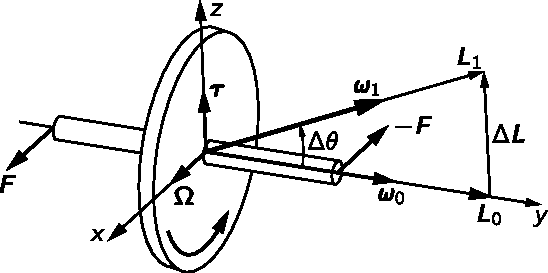
\includegraphics[width=0.3\linewidth]{fyz_fig407.pdf}
    \caption{Setrvačník
             (\cite[s.~279]{Feynman01})}
    \label{fyz:fig407}
  \end{figure}

  \begin{figure}[ht!] %\ref{fyz:fig408}
    \centering
    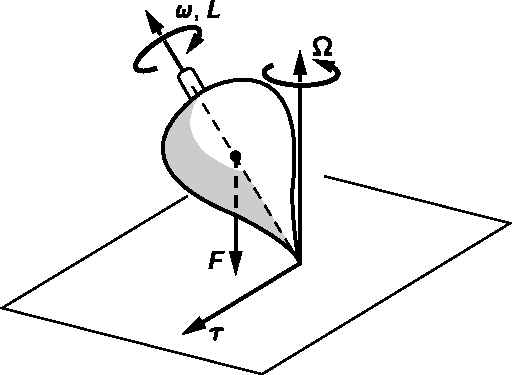
\includegraphics[width=0.3\linewidth]{fyz_fig408.pdf}
    \caption{Rychle se otáčející káča. Směr vektoru momentu síly je směrem precese 
             (\cite[s.~280]{Feynman01})}
    \label{fyz:fig408}
  \end{figure}

  \begin{figure}[ht!] %\ref{fyz:fig409}
    \centering
    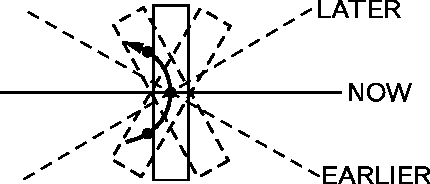
\includegraphics[width=0.3\linewidth]{fyz_fig409.pdf}
    \caption{Při otáčení osy vykonávají částice rotujícího kola (obr. \ref{fyz:fig407}) pohyb, 
             který se děje po zakřivených trajektoriích 
             (\cite[s.~280]{Feynman01})}
    \label{fyz:fig409}
  \end{figure}

  \begin{figure}[ht!] %\ref{fyz:fig410}
    \centering
    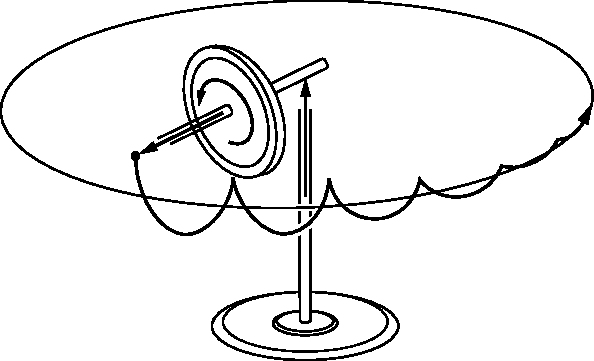
\includegraphics[width=0.3\linewidth]{fyz_fig410.pdf}
    \caption{Skutečný pohyb konce setrvačníku pod vlivem tíhy ihned po uvolnění předtím uchycené osy
             (\cite[s.~281]{Feynman01})}
    \label{fyz:fig410}
  \end{figure}

  \begin{figure}[ht!] %\ref{fyz:fig411}
    \centering
    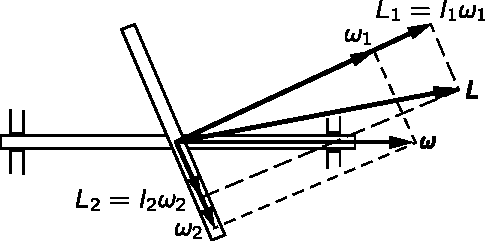
\includegraphics[width=0.3\linewidth]{fyz_fig411.pdf}
    \caption{Moment hybnosti rotujícího tělesa není nutně rovnoběný s úhlovou rychlostí
             (\cite[s.~282]{Feynman01})}
    \label{fyz:fig411}
  \end{figure}

  \begin{figure}[ht!] %\ref{fyz:fig412}
    \centering
    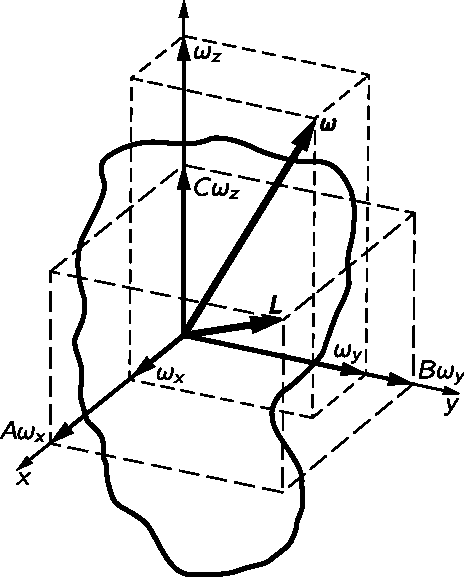
\includegraphics[width=0.3\linewidth]{fyz_fig412.pdf}
    \caption{Úhlová rychlost a moment hybnosti tuhého tělesa (\(A>B>C\))
             (\cite[s.~283]{Feynman01})}
    \label{fyz:fig412}
  \end{figure}

  \todo[inline]{Kapitola fey1ch20 je zcela prázdná, pouze obrázky}  
%} %tikzset
%---------------------------------------------------------------------------------------------------